\documentclass[25pt, a0paper, portrait, margin=0mm, innermargin=15mm,
     blockverticalspace=15mm, colspace=15mm, subcolspace=8mm]{tikzposter}
\usetheme{Wave}
\useblockstyle{TornOut}
\usenotestyle{Sticky}

\makeatletter
\def\title#1{\gdef\@title{\scalebox{\TP@titletextscale}{%
\begin{minipage}[t]{\linewidth}
\centering
#1
\par
\vspace{0.5em}
\end{minipage}%
}}}
\makeatother

\makeatletter
\newcounter{tablecounter}
\newenvironment{tikztable}[1][]{
  \def \rememberparameter{#1}
  \vspace{10pt}
  \refstepcounter{tablecounter}
  \begin{center}
  }{
    \ifx\rememberparameter\@empty
    \else
    \\[10pt]
    {\small Table~\thetablecounter: \rememberparameter}
    \fi
  \end{center}
}
\makeatother

\usepackage{booktabs}
\usepackage{array}
\usepackage{graphicx}  % package for inserting images, including .pdf
\usepackage{adjustbox} % package for cropping images
\usepackage[colorlinks=true, urlcolor=orange]{hyperref} % package for url and hyperlinks
\usepackage{wrapfig}

\title{Assessing United States county-level exposure for 
  hurricane and tropical storm  epidemiological research}
\author{Brooke Anderson*, Joshua Ferreri, Mohammad Al-Hamdan, William Crosson, Andrea Schumacher, Seth Guikema, Steven Quiring, Dirk Eddelbuettel, Meilin Yan, Roger Peng}
\institute{*Colorado State University, Fort Collins, CO, USA \\[0.5cm] 
E-mail: \texttt{\href{mailto:brooke.anderson@colostate.edu}{brooke.anderson@colostate.edu}}}

\begin{document}

\maketitle

\begin{columns}

%% Left column
\column{0.33}

% Summary block
\block{1. Motivation}{
Hurricanes and other tropical storms bring severe impacts to U.S. communities. These impacts can result from a variety of storm-related hazards, including extreme wind, rain, flooding, and tornadoes. Epidemiological studies vary widely in how they classify \textbf{exposure to tropical cyclones}, using various hazard-based metrics and, in some cases, using distance from the storm as a surrogate for exposure to storm-related hazards. 

} % Closes block 1, Summary

\block{2. Identifying storm exposures}{

Here we measure county-level exposure to tropical cyclones in the United States based on several of these metrics for Atlantic basin storms for 1996--2011 (Table 1). \\[0.01cm] 

\coloredbox{
% Exposure definition table
\small
\begin{tikztable}[Criteria for tropical cyclone exposures]
\begin{tabular}{p{3cm}p{19cm}} 
\toprule
Metric &  Criteria for exposure \\ \midrule 
\textbf{Distance} &  County population mean center within 100 kilometers of storm track \\ 
\textbf{Rain} &  County cumulative rainfall of 75 millimeters or more over the period from two days before to one day after the storm's closest approach and county population mean center within 500 kilometers of the storm track \\ 
\textbf{Wind} &  Modeled maximum sustained wind speed at the county's population mean center 15 meters per second or higher during the storm\\ 
\textbf{Flood} &  Flood event listed in the National Oceanic and Atmospheric Administration (NOAA) Storm Events database for the county with a start date within two days of the storm's closest approach and county population mean center within 500 kilometers of the storm track \\
\textbf{Tornado} &  Tornado event listed NOAA Storm Events database for the county with a start date within two days of the storm's closest approach and county population mean center within 500 kilometers of the storm track\\
\bottomrule 
\end{tabular} 
\end{tikztable}
}

\medskip

We considered all tracked storms in the revised Atlantic
hurricane database (HURDAT2).
For the \textbf{rain}-based exposure metric, cumulative rainfall was estimated from two days before to one day after the storm's closest
approach to the county, using North American Land Data
Assimilation System Phase 2 (NLDAS-2) data. 
For the \textbf{wind}-based exposure metric, we modeled maximum sustained wind
speeds at each county's population mean center.
To identify \textbf{flood}- and \textbf{tornado}-based exposures to tropical cyclones in U.S.
counties, we used event listings from the National Oceanic and Atmospheric
Administration's Storm Event Database. \\[0.01cm]
  
  % Sub-block with R package information
  \innerblock{R package \texttt{hurricaneepxosure}}{
  
To assist with future tropical cyclone epidemiological studies, we created 
the R package \textbf{hurricaneexposure}, which is
open source software with hazard-specific, county-level tropical
cyclone exposure data, as well as tools to explore and map the data.
  }

} % Closes block 2, identifying tropical cyclone exposures

\block{3. Measuring agreement}{

We
measured agreement between exposure metrics by calculating
the within-storm \textbf{Jaccard index} between every pair-wise combination of metrics. The
Jaccard index ($J_s$) measures similarity between two metrics ($X_{1,s}$ and
$X_{2,s}$) for storm $s$ as the proportion of counties in which both of the
metrics classify the county as exposed, out of all counties classified as exposed
by at least one of the metrics:

\begin{equation} 
J_s = \frac{X_{1,s} \cap X_{2,s}}{X_{1,s} \cup X_{2,s}}
\end{equation}

} % Closes block 3., measuring agreement between metrics

%% Right column
\column{0.67}

\block{4. Agreement among exposure classifications}{


  % Sub-block with Ivan example
  \innerblock{Agreement for one example storm: Hurricane Ivan (2004)}{
  \begin{wrapfigure}[20]{r}{0.68\colwidth}
    \begin{tikzfigure}[Counties classified as exposed to Hurricane Ivan (2004) 
                       (orange) based on each exposure metric. The red line shows 
                       the track of Hurricane Ivan based on the revised Atlantic
                       hurricane database (HURDAT2).] 
    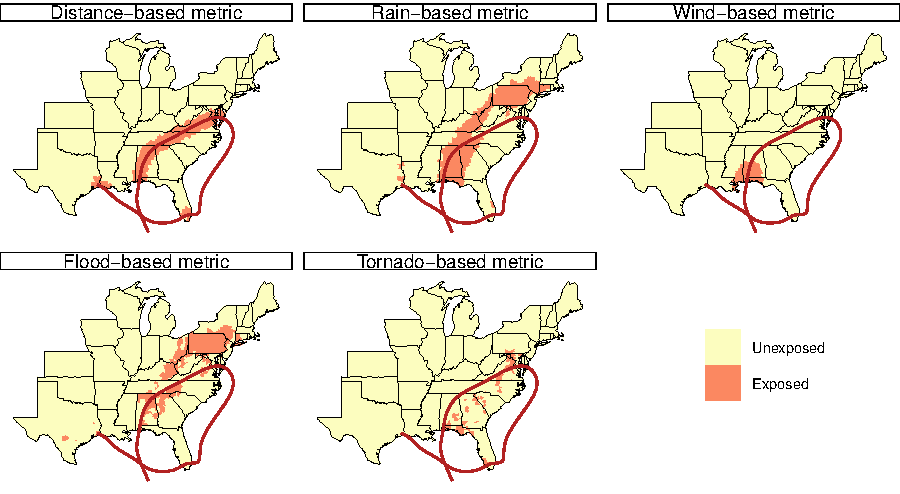
\includegraphics[width = 0.68\colwidth]{../figures/ivanonly}
    \end{tikzfigure} 
  \end{wrapfigure}
  We found that switching among these metrics can dramatically change which counties are identified as exposed to a particular storm.
Fig. 1 gives an example for Hurricane Ivan (2004). When county-level exposure was determined based on
the \textbf{wind} metric, only counties near two of the storm's landfalls were assessed
as exposed. For \textbf{rain}- and \textbf{flood}-based metrics, however, exposure extended to the
left of the track, including counties as far north as New York and Connecticut,
while for the \textbf{tornado} metric, exposed counties tended to be to the right of the
track and included several counties not identified as exposed by any other
metric.
  }
  
  \vspace{0.5cm}
  
  % Sub-block with Jaccard agreement
  \innerblock{Agreement for all major storms}{
  
  \begin{wrapfigure}[18]{l}{0.45\colwidth}
  \begin{tikzfigure}[Jaccard index values for
agreement between exposure metric pairs for major storms, 1996--2011.]
  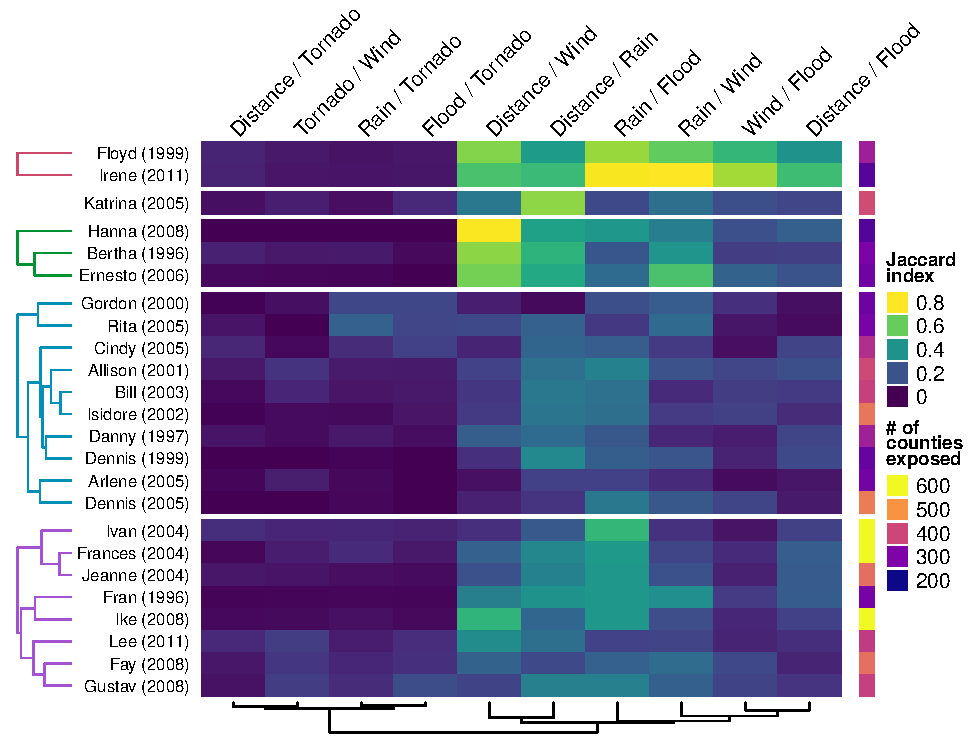
\includegraphics[width=0.45\colwidth]{../figures/jaccard_heatmap_presentation.pdf}
  \end{tikzfigure}
  \end{wrapfigure}
 
   We drew similar conclusions when we investigated all 24 storms for which 250 or
more counties were exposed based on at least one metric (Fig.
2). The color of each cell within the main heatmap indicates the Jaccard index for a given pair
of metrics for a given storm. Storms are displayed within clusters that have
similar patterns in county-level exposure agreement for metric pairs. The colors to the right of
the main heatmap for each storm indicate the total number of counties classified
as exposed to the storm by any of the five metrics. 

The tornado-based metric showed universally poor agreement
with other metrics in county-level classification across all storms considered.
For other pairs of metrics, there were also \textbf{generally large differences} in
which counties were determined to be exposed to the storm, with the Jaccard
index values below 0.4 for most metric pairs in most storms.


There were, however, \textbf{a few exceptions}---storms in which similar counties were
determined to be exposed to the storm for two or more of the metrics
considered.  For Floyd (1999) and Irene (2011), for example, county-level
classification agreed moderately to well (Jaccard index of approximately
0.5--0.8) for all pairs of exposure metrics except those including the
tornado-based metric. These storms both made their first U.S. landfall in North
Carolina at minor hurricane windspeeds (Category 2 and 1, respectively) and
then skimmed the eastern coast of the U.S. north through New England, bringing
large rainfall to much of the eastern coast from North Carolina north and
causing extensive inland flooding in North Carolina (Floyd) and New England
(Irene).
  }

} % Closes block 4, Agreement among exposure classification

\block{5. Conclusions}{

Previous research has highlighted the range of impacts that tropical cyclones
can have in US communities. 
Determining the metrics of storm exposure that are most
associated with loss of life, property damage, and other impacts may help
identify and quantify the important threats that remain from tropical cyclones
in the US, which could allow future success in reducing these threats through
community planning, warning systems, and other measures. Locations identified as storm-exposed varied substantially when switching among metrics based on different storm hazards, and distance to the storm was at best a moderate, and often a poor, surrogate for storm hazard exposures. Therefore, when impact studies use distance as a surrogate of exposure to tropical cyclone exposures or use one hazard-based metric (e.g., wind-based) when the impact is partly or fully caused by a different storm hazard (e.g., flooding), the analysis will be prone to exposure misclassification, which can mask true associations. To facilitate future research, we make multi-hazard storm exposure data for the US available through open-source software.

}

\note[angle=270, radius=9cm, width=50cm, innersep=1cm]{
\small  
\textbf{Acknowledgements.} 
This work was supported in part by grants from the National Institute of
Environmental Health Sciences (R00ES022631), the National Science Foundation
(1331399), the Department of Energy (Grant No. DE-FG02-08ER64644), and a
National Aeronautics and Space Administration Applied Sciences Program/Public
Health Program Grant (NNX09AV81G). Rainfall data are based on data acquired as
part of the mission of the National Aeronautics and Space Administration's Earth
Science Division and archived and distributed by the Goddard Earth Sciences
(GES) Data and Information Services Center (DISC).
  
} % Closes Acknowledgements block

\end{columns}

\end{document}